% VLDB template version of 2020-03-05 enhances the ACM template, version 1.7.0:
% https://www.acm.org/publications/proceedings-template
% The ACM Latex guide provides further information about the ACM template

\documentclass{article}
\usepackage{listings}
\usepackage[margin=20mm]{geometry}
\usepackage{graphicx}
\usepackage{amsfonts}
\usepackage{amsmath}
\usepackage{physics}
\usepackage{parskip}
\usepackage{enumitem}
\usepackage{cancel}

%% The following content must be adapted for the final version
% paper-specific
\newcommand\vldbdoi{XX.XX/XXX.XX}
\newcommand\vldbpages{XXX-XXX}
% issue-specific
\newcommand\vldbvolume{14}
\newcommand\vldbissue{1}
\newcommand\vldbyear{2020}
% should be fine as it is
\newcommand\vldbauthors{\authors}
\newcommand\vldbtitle{\shorttitle} 
% leave empty if no availability url should be set
\newcommand\vldbavailabilityurl{http://vldb.org/pvldb/format_vol14.html}
\newcommand\oname{\operatorname}

\newtheorem{theorem}{Teor.}
\newtheorem{definition}{Def.}
\newtheorem{example}{Ej.}
\newtheorem{excercise}{Ejer.}

\begin{document}

\textbf{Ex. 2.1: }Is it possible to find a general formula for $p(C|A+B)$, analogous to $(2-48)$, from the product and sum rules? If so, derive it; if not, explain why this cannot be done.

\textbf{Answer:}

Sure. We've derived Bayes theorem without naming it, which is simply product rule and commutativity, so we can say
\begin{align*}
	p(C|A+B)&=\frac{p(C)\,p(A+B|C)}{p(A+B)}\\
	&=\frac{p(C)\,\left(p(A)+p(B)-p(AB|C)\right)}{p(A)+p(B)-p(AB)}.
\end{align*}

\textbf{Ex. 2.2: }Now suppose we have a set of propositions $\{A_1,\,\cdots,\,A_n\}$ which on information $X$ are mutually exclusive: $p(A_iA_j|X)=p(A_i|X)\delta_{ij}$. Show that $p(C|(A_1+A_2+\cdots+A_n)X)$ is a weighted average of the separate plausibilities $p(C|A_iX)$:
\begin{align*}
	p(C|(A_1+\cdots+A_n)X)=p(C|A_1X+A_2X+\cdots+A_nX)=\frac{\sum_ip(A_i|X)p(C|A_iX)}{\sum_ip(A_i|X)}.
\end{align*}

\textbf{Answer:}
For $i\neq j$,
\begin{align*}
	p(C|A+B)&=\frac{p(A+B|C)p(C)}{p(A+B)}\\
	&=\frac{(p(A)+p(B)-p(AB|C))p(C)}{p(A)+p(B)-p(AB|C)}.
\end{align*}
Iterating this over $\sum_iA_i$ we get
\begin{align*}
	p\left(\sum_iA_i\middle|X\right)&=\sum_ip(A_i|X).
\end{align*}

Thus, and in a similar manner to the above excercise,
\begin{align*}
	p\left(C\middle|\sum_iA_iX\right)&=\frac{p\left(\sum_iA_i\middle|CX\right)p(C|X)}{p(\sum_iA_i|X)}\\
	&=\frac{\sum_ip(A_i|CX)p(C|X)}{\sum_ip(A_i|X)}\\
	&=\frac{\sum_ip(A_i|X)p(C|A_iX)}{\sum_ip(A_i|X)}.
\end{align*}

\textbf{Ex.: }Let $A_i$ mutually exclusive ($P(A_iA_j)=P(A_i)\delta_{ij}$). Then, $P(\sum_iA_i)=\sum_iP(A_i)$.

\textbf{Answer: }

If $i\in\{1,\,2\}$, then
\begin{align}
	P(\sum_iA_i)&=P(A_1+A_2)\\
	&=P(A_1)+P(A_2)-\cancelto0{P(A_1A_2)}\\
	&=\sum_iP(A_i).
\end{align}

Then, by induction,
\begin{align}
	P\left(\sum_i^{N+1}A_i\right)&=P\left(\sum_i^NA_i\right)+P(A_{N+1})-P\left(\sum_i^NA_iA_{N+1}\right)\\
	&=\sum_i^NP(A_i)+P(A_{N+1})-\sum_i^N\cancelto0{(A_iA_{N+1})}\\
	&=\sum_iP(A_i).
\end{align}

\textbf{Ex. 2.3: Limits on Probability Values: } As soon as we have the numerical values $a=P(A|C)$ and $b=P(B|C)$, the product and sum rules place some limits on the possible numerical values for their conjunction and disjuncion. Supposing that $a\leq b$, show that the probability of the conjunction cannot exceed that of the least possible proposition: $0\leq P(AB|C)\leq a$, and the probability of the disjunction cannot be less than that of the most probable proposition: $b\leq P(A+B|C)\leq 1$. Then show that, if $a+b>1$, there is a stronger inequality for the conjunction; and if $a+b<1$ there is a stronger one for the disjunction. These necessary general inequalities are helpful in detecting errors in calculations.

\textbf{Answer: }

For the conjunction,
\begin{align}
	P(AB|C)&=P(A|C)P(B|AC)\\
	&=aP(B|AC)
	&\leq a.
\end{align}

Since $P(AB|C)=b+a-P(A+B|C)$, if $b+a>1$ then $P(AB|C)>1-P(A+B|C)=P(\overline{A+B}|C)$.

For the disjunction,
\begin{align}
	P(A+B|C)&=P(A|C)+P(B|C)-P(AB|C)\\
	&=b+a-P(AB|C)\\
	&\geq b.
\end{align}

And also, $b+a<1$ implies $P(A+B|C)<1-P(AB|C)=P(\overline{AB}|C)$.

\textbf{Ex. 3.1: }Why isn't the multiplicity factor $(3-16)$ just $n!$? After all, we started this discussion by stipulating that the balls, in addition to having colors, also carry labels $(1\cdots N)$, so that different permutations of the red balls among themselves, which give the $r!$ in the denominator of $(3-16)$, are distinguishable arrangements.

\textbf{Answer: }

We've decomposed the event ``drawing $r$ red balls in $n$ draws'' as the union of events of the form ``draw $r$ red balls in $n$ draws with the particular permutation of orders $p$'' for permutations $p$, which are mutually exclusive and identically plausible. At doing this, we're using the events $R_i$ and $W_i$, with the probability given by $(3-14)$. If we were to use ``drawing the following $n$ balls, where $r$ are red'', we should be accounting for the probability $B_{ij}$ of drawing the $i$th ball after $j$ draws, which would incorporate the missing factors.

\textbf{Ex. 3.2: Probability of a Full Set: }Suppose an urn contains $N=\sum_iN_i$ balls, $N_1$ of color $1$, $N_2$ of color $2$, $\cdots$, $N_k$ of color $k$. We draw $m$ balls without replacement; what is the probability that we have at least one of each color? Supposing $k=5$, all $N_i=10$, how many do we need to draw in order to have at least $90\%$ probability of getting a full set?

\textbf{Answer: }

We're asked $P\left(\sum_{r\in I}\prod_ir_i\right)$, where $I=\{(r_i):\,r_i\geq1\forall i\}$. We can decompose this as 
\begin{align}
	P\left(\sum_{r\in I}\prod_ir_i|B\right)&=\sum_{r\in I}P\left(r_1\cdots r_k|B\right)\\
	&=\frac1{\begin{pmatrix}N\\m\end{pmatrix}}\sum_{r\in I}\prod_i\begin{pmatrix}N_i\\r_i\end{pmatrix}
\end{align}

A calculation is probably better done by calculating the missing terms instead, which are those for which at least one of those are $0$, of which there are less, since at least one of the summands is already $0$, the rest varying between the same intervals.

The ``3.2.py'' script does the maths, and outputs $m=15$ as the solution, with a probability of about $0.91$.

\textbf{Ex. 3.3: Reasoning Backwards: }Suppose that in the previous exercise $k$ is initially unknown, but we know that the urn contains exactly $50$ balls. Drawing out $20$ of them, we find $3$ different colors; now what do we know about $k$? We know from deductive reasoning (i.e., with certainty) that $3\leq k\leq 33$; but can you set narrower limits $k_1\leq k\leq k_2$ within which it is highly likely to be?

\textbf{Answer:}

I suppose this is the first use case of Bayes theorem as it's usually used. By letting the hypotheses $H_k=\text{``There are $k$ different colors in the urn''}$ and the data $D=\text{``3 different colors have been seen after 20 draws''}$, we want $P(H_k|D)$, but what our model tells us with certainty is $P(D|H_k)$, so we'll use Bayes' theorem for this:
\begin{align}
	P(H_k|D)&=\frac{P(D|H_k)P(H_k)}{\sum_kP(D|H_k)P(H_k)}.
\end{align}
I will assume each $H_k$ is equally likely, since I've got no information on anything. Thus,
\begin{align}
	P(H_k|D)&=\frac{P(D|H_k)}{\sum_kP(D|H_k)}.
\end{align}

We're now left with the task of finding the probability that $3$ different colors are seen in a set of $20$ taken from $50$, given there are $k$ different colors. To this end, we split $D=\sum_NDH_N$, where $N\in\mathbb N^k$ is such that $N_i$ is the number of balls with the $i$th color, and get
\begin{align}
	P(D|H_k)&=P\left(\sum_NDH_N\middle|H_k\right)\\
	&=\sum_NP(DH_N|H_k)\\
	&=\sum_NP(D|H_NH_k)P(H_N|H_k).
\end{align}
We once again propose an homogeneous distribution over the $N$, which gives $P(H_N|H_k)=\begin{pmatrix}50-k\\k-1\end{pmatrix}^{-1}$.

Now, let's think of the probability of drawing from only the colors $1$, $2$, and $3$ in all draws. For the $m$th draw, the probability is
\begin{align}
	\frac{51-m-\sum_{l=3}^{k-2}N_l}{51-m}&=\frac{51-m-N_\text{rem}}{51-m},
\end{align}
so for the 20 draws, we get
\begin{align}
	\frac{\left(50-N_\text{rem}\right)!\;30!}{\left(30-N_\text{rem}\right)!\;50!}.
\end{align}

So, the chances of drawing only the first $3$ colors are the sum over all of the $N$ of this term. For each choice of $N_\text{rem}$, there are $\begin{pmatrix}47-N_\text{rem}\\2\end{pmatrix}=(47-N_\text{rem})(46-N_\text{rem})$ such terms. And, by simmetry of label permutation, for each choice of $3$ colors the result is the same, so finally, by splitting $D$ into the sum of ``drawing only for these $3$ particular colors'', we sum over these $k!/(k-3)!$ choices, and get our final result:
\begin{align}
	P(D|H_k)&=\frac{k!}{(k-3)!}\sum_{N_\text{rem}=k-3}^{47}(47-N_\text{rem})(46-N_\text{rem})\frac{(50-N_\text{rem})!\;30!}{(30-N_\text{rem})!\;50!}\begin{pmatrix}50-k\\k-1\end{pmatrix}^{-1}
\end{align}

The ``3.3.py'' script implements this solution, giving the probability distribution shown in Figure \ref{fig:3.3}
\begin{figure}[h]
	\center
	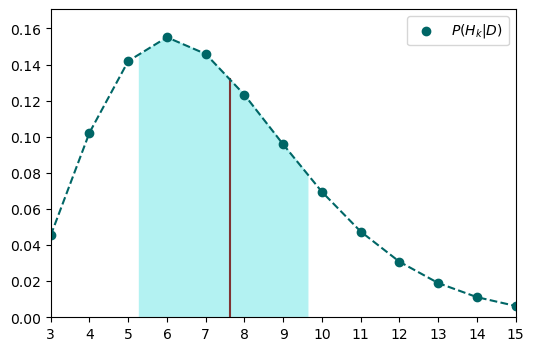
\includegraphics[width=0.5\textwidth]{Numerical/3.3.png}
	\caption{Probability distribution $P(H_k|D)$ for different values of $k$. The shaded region goes between first and third quartile, and the vertical line denotes the (linearly extrapolated) median.}
	\label{fig:3.3}
\end{figure}

\textbf{Ex. 3.4: Matching: }The $M$ urns are now numbered $1$ to $M$, and $M$ balls, also numbered $1$ to $M$, are thrown into them, one in each urn. If the numbers of a ball and its urn are the same, we have a match. Show that the probability of at least one match is
\begin{align*}
	P&=\sum_{k=1}^M(-1)^{k+1}/k!.
\end{align*}

As $M\rightarrow\infty$, this converges to $1-1/e=0.632$. The result is surprising to many, because however large $M$ is, there remains an appreciable probability of no match at all.

\textbf{Answer:}

I give up. The problem turns out to be that of counting derangements, which Wikipedia explains:

Let the urn $1$ receive ball $i$. If urn $i$ receives ball $1$, then we're left with the problem of counting derangements for $M-2$.
If urn $i$ receives a ball other than $1$, then it's the problem of counting derangements for $M-1$, since for each of the other urns there is $1$ ball they may not receive (urn $i$ shall not receive ball $1$). Thus,
\begin{align}
	!n&=(n-1)(!(n-1)+!(n-2)),
\end{align}
which may now be solved by induction.

\textbf{Ex. 3.5: Occupancy: }$N$ balls are tossed into $M$ urns; there are evidently $M^N$ ways this can be done. If the robot considers them all equally likely, what is its probability that each urn receives at least one ball?

\textbf{Answer: }

If they're equally likely, we can just count. We'll count the negative, summing over the number $k$ of boxes with no matches. There are $\begin{pmatrix}M\\k\end{pmatrix}$ such choices, and the rest of boxes allow for $(M-k)^N$ choices, so there are
\begin{align}
	\sum_{k=1}^M\begin{pmatrix}M\\k\end{pmatrix}(M-k)^N
\end{align}
instances where no box receives balls, and thus
\begin{align}
	P(\text{``Each urn receives at least one ball''})&=1-\sum_{k=1}^M\begin{pmatrix}M\\k\end{pmatrix}\left(1-\frac{k}{M}\right)^N
\end{align}

\textbf{Ex. 4.1: }Show that there is no such nontrivial extension of the binary case. More specifically, prove that if $(4.28)$ and $(4.29)$ hold with $n>2$, then at most one of the factors
\begin{align*}
	\frac{P\left(D_1\middle|H_i\,X\right)}{P\left(D_1\middle|\overline{H_i}\,X\right)}\cdots\frac{P\left(D_m\middle|H_i\,X\right)}{P\left(D_m\middle|\overline{H_i}\,X\right)}
\end{align*}
is different from unity, therefore at most one of the data sets $D_j$ can produce any updating of the probability for $H_i$.

\textbf{Answer:}

The equations mentioned are that of independence in $D_1$ to $D_m$ conditioned to both the hypothesis and its negation:
\begin{align*}
	P\left(D_1,\ldots,D_m\middle|A\,X\right)&=\prod_jP\left(D_j\middle|A\,X\right)\;\;\forall A\in\{H_i,\,\overline{H_i}\}\forall i\in[1,n]_{\mathbb N},
\end{align*}
under the hypothesis that the $H_i$ are exhaustive.

This means
\begin{align*}
	P(H_i|D_j\,X)+P\left(\overline{H_i}\middle|D_j\,X\right)&=1,\\
	\left(P(D_j|H_i\,X)-P\left(D_j\middle|\overline{H_i}\,X\right)\right)P(H_i|X)&=P(D_j|X)-P\left(D_j\middle|\overline{H_i}\,X\right).
\end{align*}

I believe the proof has to do with the fact that, for a proposition $D_j$ such that $P(D_j|H_i\,X)\neq P\left(D_j\middle|\overline{H_i}\,X\right)$,
\begin{align*}
	P(H_i|X)&=\frac{P(D_j|X)-P\left(D_j\middle|\overline{H_i}\,X\right)}{P(D_j|H_i\,X)-P\left(D_j\middle|\overline{H_i}\,X\right)},
\end{align*}
but so far it's leading me nowhere.

Maybe use that
\begin{align*}
	P(D_k|\overline{H_i})-P(D_k|H_i)&=\sum_{j\neq i}\frac{P(D_k|H_j)P(H_j)}{P(\overline{H_i})}-P(D_k|H_i)\\
	&=\frac1{P(\overline{H_i})}\sum_j\left[P(D_k|H_j)-P(D_k|H_i)\right]P(H_j),\\
	\left[P(D_k|\overline{H_i})-P(D_k|H_i)\right]_k&=\frac1{P(\overline{H_i})}\left[P(D_k|H_j)-P(D_k|H_i)\right]_{kj}\left[P(H_j)\right]_j
\end{align*}

% TODO: Solve this

\textbf{Ex. 4.2: }Calculate the exact threshold of skepticism $f_t(x,\,y)$, supposing that proposition $C$ has instead of $10^{-6}$ an arbitrary prior probability $P(C|X)=x$, and specifies instead of $99/100$ an arbitrary fraction $y$ of bad widgets. Then discuss how the dependence on $x$ and $y$ corresponds - or fails to correspond - to human common sense.

\textbf{Answer:}

Okay, let's do this.

% This section is commented. It's a recap.
Evidence is defined by
\begin{align*}
	e(H|DX)&=10\log_{10}O(H|DX)\\
	&=10\log_{10}\left[\frac{P(H|DX)}{P(\overline{H}|DX)}\right]\\
	&=10\log_{10}\left[\frac{P(D|HX)P(H|X)}{P(D|\overline{H}X)P(\overline{H}|X)}\right]\\
	&=e(H|X)+10\log_{10}\left[\frac{P(D|HX)}{P(D|\overline{H}X)}\right].
\end{align*}

So, for multiple mutually exclusive and exhaustive hypotheses,
\begin{align*}
	e(H_i|DX)&=e(H_i|X)+10\log_{10}\left[\frac{P(D|H_iX)}{P(D|\sum_{j\neq i}H_jX)}\right],
\end{align*}
and we can replace
\begin{align}
	P\left(D\middle|\sum_{j\neq i}H_jX\right)&=P\left(D\sum_{k\neq i}H_j\middle|\sum_{j\neq i}H_jX\right)\\
	&=\sum_{k\neq i}\frac{P(DH_k\sum_{j\neq i}H_j|X)}{P(\sum_{j\neq i}H_j|X)}\\
	&=\frac{\sum_{k\neq i}P(DH_k|X)}{\sum_{j\neq i}P(H_j|X)}\\
	&=\frac{\sum_{k\neq i}P(D|H_kX)P(H_k|X)}{\sum_{k\neq i}P(H_k|X)}.
\end{align}

So, letting $w_k^{(i)}=P(H_k|X)/\sum_{j\neq i}P(H_j|X)$,
\begin{align*}
	e(H_i|DX)&=e(H_i|X)+10\log_{10}\left[\frac{P(D|H_iX)}{\sum_{k\neq i}w_k^{(i)}P(D|H_kX)}\right].
\end{align*}

This is, we're comparing the likelihood of $H_i$ with the sum of the likelihoods $H_k$ for $k\neq i$ weighted by their prior likelihood. So yeah, I guess we can keep the $j$th term of the denominator as long as it's $10$ times bigger than the rest of them.

In the problem at hand,
\begin{align*}
	P(A|X)=\frac1{11}(1-x),\\
	P(B|X)=\frac{10}{11}(1-x),\\
	P(C|X)=x.
\end{align*}

Furthermore, if after $m$ measurements we find $fm$ of them are bad,
\begin{align*}
	P(D|AX)&=\left(\frac13\right)^{fm}\left(\frac23\right)^{(1-f)m},\\
	P(D|BX)&=\left(\frac16\right)^{fm}\left(\frac56\right)^{(1-f)m},\\
	P(D|CX)&=y^{fm}(1-y)^{(1-f)m}.
\end{align*}

This all results in
\begin{align*}
	e(C|DX)&=e(C|X)+10\log_{10}\left[\frac{P(D|CX)}{w_A^{(C)}P(D|AX)+w_B^{(C)}P(D|AX)}\right]\\
	&=10\log_{10}\left[\frac{x}{1-x}\right]+10\log_{10}\left[\frac{y^{fm}(1-y)^{(1-f)m}}{\frac1{11}\left(\frac13\right)^{fm}\left(\frac23\right)^{(1-f)m}+\frac{10}{11}\left(\frac16\right)^{fm}\left(\frac56\right)^{(1-f)m}}\right]\\
	&=10\log_{10}\left[\frac{x}{1-x}\right]+10\log_{10}\left[\frac{\left(\left(\frac{y}{1-y}\right)^f(1-y)\right)^m}{\frac1{11}\left(\left(\frac12\right)^f\frac23\right)^m+\frac{10}{11}\left(\left(\frac15\right)^f\frac56\right)^m}\right].
\end{align*}

I find the last form more enlightening for the problem at hand. All of those terms are of the form $\text{something}^m$. For $m\rightarrow\infty$, the term with the higher base will govern the denominator. To see which, we note the quotient of them is
\begin{align*}
	\left(\frac52\right)^f\frac45,
\end{align*}
so setting this to unity yields a critical value $f=\log\left(\frac54\right)/\log\left(\frac52\right)\approx0.24$. Given that the term in parentheses is greater than one, this means hypothesis $A$ governs when $f$ goes above this value, and $B$ governs otherwise. If we want the threshold for $y>\frac13$, it is clear that we need to work in the range where hypothesis $A$ is more likely. So the threshold of skepticism is given by the value $f$ such that the quotient
\begin{align*}
	\left(2\frac{y}{1-y}\right)^f\frac32(1-y)
\end{align*}
is equal to $1$. This yields the exact value
\begin{align*}
	f_t(x,\,y)&=\frac{\log\left(\frac23\frac1{1-y}\right)}{\log\left(2\frac{y}{1-y}\right)}.
\end{align*}

For $y=99/100$, this yields approximately $0.794155$, in conflict with the value of $0.793951$ given in the book. But the solution book I'm contrasting with in github gives this same value, $0.7941$etc.

The general case for estimating this threshold is now obvious:
\begin{align*}
	f_t&=\frac{\log\left[\frac{P(\text{good}|CX)}{P(\text{good}|AX)}\right]}{\log\left[\frac{P(\text{bad}|CX)P(\text{good}|AX)}{P(\text{good}|CX)P(\text{bad}|AX)}\right]}.
\end{align*}

\textbf{Ex. 4.3: }Show how to make the robot skeptical about both unexpectedly high and unexpectedly low numbers of bad widgets in the observed sample. Give the full equations. Note particularly the following: if $A$ is true, then we would expect, according to the binomial distribution ($3.86$), that the observed fraction of bad ones would tend to about $1/3$ with many tests, while if $B$ is true it should tend to $1/6$. Suppose that it is found to tend to the threshold value ($4.24$), close to $1/4$. On sufficiently large $m$, you and I would then become skeptical about $A$ and $B$; but intuition tells us that this would require a much larger $m$ than ten, which was enough to make us and the robot skeptical when we find them all bad. Do the equations agree with our intuition here, if a new hypothesis $F$ is introduced which specifies $P(\text{bad}|F\,X)\approx1/4$?

\textbf{Answer:}

Let us devise hypotheses $C$ and $E$, pertaining chances $99/100$ and $1/100$ of bad widgets. We thus have, for a certain hypothesis $H\in\{A,\,B,\,C,\,E\}$,
\begin{align*}
	e(H|D\,X)&=e(H|X)+10\log_{10}\left[\frac{P(D|H\,X)}{\sum_{H'\neq H}w_{H'}^{(H)}P(D|H'\,X)}\right],
\end{align*}
with
\begin{align*}
	P(D|H\,X)&=\left[P(\text{bad}|H\,X)\right]^{m_b}\left[1-P(\text{bad}|H\,X)\right]^{m-m_b}\\
		 &=\left(\left[\frac{P(\text{bad}|H\,X)}{1-P(\text{bad}|H\,X)}\right]^{m_b/m}\left[1-P(\text{bad}|H\,X)\right]\right)^m.
\end{align*}

It is then evident that the relevant comparison is between the terms in parentheses. Namely, we're concerned with
\begin{align*}
	\left(\frac{P(D|H\,X)}{P(D|H'\,X)}\right)^{1/m}&=\left(\frac{P(\text{bad}|H\,X)}{P(\text{bad}|H'\,X)}\right)^{m_b/m}\left(\frac{P(\text{good}|H\,X)}{P(\text{good}|H'\,X)}\right)^{m_g/m}\\
	&=\left(\frac{P(\text{bad}|H\,X)}{P(\text{bad}|H'\,X)}\frac{(1-P(\text{bad}|H'\,X))}{(1-P(\text{bad}|H\,X))}\right)^{m_b/m}\frac{1-P(\text{bad}|H\,X)}{1-P(\text{bad}|H'\,X)},
\end{align*}
which gives the general threshold
\begin{align*}
	f(H,\,H')&=\frac{\log\left[\frac{P(\text{good}|H'\,X)}{P(\text{good}|H\,X)}\right]}{\log\left[\frac{P(\text{bad}|H\,X)}{P(\text{bad}|H'\,X)}\frac{P(\text{good}|H'\,X)}{P(\text{good}|H\,X)}\right]}.
\end{align*}
In case the symmetry ain't evident, you can see that
\begin{align*}
	f(H,\,H')&=\frac{\log P(\text{good}|H'\,X)-\log P(\text{good}|H\,X)}{\log\left[\frac{P(\text{bad}|H\,X)}{P(\text{good}|H\,X)}\right]-\log\left[\frac{P(\text{bad}|H'\,X)}{P(\text{good}|H'\,X)}\right]}.
\end{align*}

Intuition tells that this value is between the rates $f_H=P(\text{bad}|H\,X)$ and $f_{H'}=P(\text{bad}|H'\,X)$, which can be seen to be true as follows. For simplicity, suppose $P(\text{bad}|H\,X)>P(\text{bad}|H'\,X)$, and observe that the quotient $\left(P(D|H\,X)/P(D|H'\,X)\right)^{1/m}$ is monotonously increasing on $m_b/m$. Further, we see that this threshold is already reached if $m_b/m=f_H$, since the function $x\mapsto x^{f_H}(1-x)^{1-f_H}$ has a maximum at
\begin{align*}
	f_Hx^{f_H-1}(1-x)^{1-f_H}+(1-f_H)x^{f_H}(1-x)^{-f_H}&=0,\\
	f_H\frac{1-x}{x}+(1-f_H)&=0,\\
	x=f_H,
\end{align*}
so that
\begin{align*}
	\left(\frac{f_H}{f_{H'}}\right)^{f_H}\left(\frac{1-f_H}{1-f_{H'}}\right)^{1-f_H}&>1,\\
	\left(\frac{f_H}{f_{H'}}\right)^{f_{H'}}\left(\frac{1-f_H}{1-f_{H'}}\right)^{1-f_{H'}}&<1,
\end{align*}
and thus $m$ is bounded between these two values.

This all demonstrates that the introduction of hypotheses $C$ and $E$ both makes us skeptical of $A$ and $B$ whenever bad widget rates go too high or drop too low, respectively.

Now, the critical value for hypothesis $F$, that $P(\text{bad}|F)=1/4$, will be given by
\begin{align*}
	P(F|D\,X)&=P(\overline F|D\,X),\\
	P(D|F\,X)P(F|X)&=\sum_{H\neq F}P(D|H\,X)P(H|X),\\
	\left(P(\text{bad}|F\,X)^{m_b/m}P(\text{good}|F\,X)^{m_g/m}\right)^mP(F|X)&=\sum_{H\neq F}\left(P(\text{bad}|H\,X)^{m_b/m}P(\text{good}|F\,X)^{m_g/m}\right)^mP(H|X).
\end{align*}

For big $m$ this could be replaced with a pairwise comparison with the closest hypothesis, under a metric we don't know but probably differentiates more between values closer to $1/2$. So I'll lazily compare it with $1/3$:
\begin{align*}
	m&=\frac{\log\left[\frac{P(A|X)}{P(F|X)}\right]}{\log\left[\left(\frac{P(\text{bad}|F\,X)}{P(\text{good}|A\,X)}\right)^{m_b/m}\left(\frac{P(\text{good}|F\,X)}{P(\text{good}|A\,X)}\right)^{m_g/m}\right]}\\
	&=\frac{\log\left[\frac{P(A|X)}{P(F|X)}\right]}{\frac{m_b}m\log\left[\frac{P(\text{bad}|F\,X)}{P(\text{bad}|A\,X)}\right]+\frac{m_g}m\log\left[\frac{P(\text{good}|F\,X)}{P(\text{good}|A\,X)}\right]}.\\
\end{align*}
It is easily seen that the closest the predictions between hypotheses, the harder to differentiate them. The inverse of the denominator takes the value $140$ (base $10$). If we pick $P(F|X)\approx1/100$ and $P(A|X)\approx1/11$ we then get the final value of $m=134$. The numerical solution involving hypotheses $A$, $B$, and $F$ (script ````4.3.py'') yields the value $2705$... high.

\textbf{Ex. 4.6: }

I'm ommiting this one. It involves going back to chapters $3$ and $4$ and reviewing which problems can't be solved by application of a different set of rules,
\begin{align*}
	p(\overline{A})&=1-p(A),\\
	p(A+B)&=p(A)+p(B)\text{ for mutually exclusive $A$ and $B$},\\
	p(AB)&=p(A)p(B)\text{ for ``independent'' $A$ and $B$}.
\end{align*}

It is easily seen that there's no definition of $A|B$, and I don't see, in a glance, how these can be used to resolve $p(AB)$ when $AB$ are not independent.

\textbf{Ex. 5.1: }

Ommited so far. Involves assigning numerical degrees of belief in diverse affirmations. Will re-visit though.

\textbf{Ex. 5.2: }From these equations, find the exact conditions on $(x,\,y,\,a,\,b)$ for divergence on the probability scale; that is,
\begin{align*}
	\abs{P(S|DI_X)-P(S|DI_Y)}>\abs{P(S|I_X)-P(S|I_Y)}.
\end{align*}

\textbf{Answer:}

The equations Edwin is refering to concern the proposition $S$ that a certain drug is safe, with data $D$ that a certain Mr. N claimed in T.V. that the drug is unsafe. Then, Mr. X and Mr. Y both have the same degree of trust in Mr. N:
\begin{align*}
	P(D|SI_X)&=P(D|SI_Y)=a,\\
	P(D|\overline{S}I_X)&=P(D|\overline{S}I_Y)=b.
\end{align*}

Here $a<b$ makes Mr. N more likely to be telling the truth. They however differ on their initial degree of trust in the drug's safety:
\begin{align*}
	P(S|I_X)&=x,\\
	P(S|I_Y)&=y,
\end{align*}
which finaly leads to
\begin{align*}
	P(S|DI_X)&=\frac{ax}{ax+b(1-x)},\\
	P(S|DI_Y)&=\frac{ay}{ay+b(1-y)}.
\end{align*}

The condition for divergence is thus, in these terms:
\begin{align*}
	\abs{\frac{ax}{ax+b(1-x)}-\frac{ay}{ay+b(1-y)}}&>\abs{x-y}.
\end{align*}

The special case $a=b$, where Mr. N is completely untrustworthy and conveys no information on his data, we get (as seen in the book), that the data changes nothing on Mr. X and Mr. Y's opinion. This equation reflects this by having no solution: rather than converging or diverging, they remain unchanged.

In the other cases, some mathsages lead to the expresion
\begin{align*}
	ab&>\abs{(ax+b(1-x))(ay+b(1-y))}.
\end{align*}

The value inside the absolute value is quadratic on $x$ and $y$, and symmetric. We're thus dealing with a conic section symmetric about axes rotated $45°$ w.r.t. the original pair of cartesian axes. This can be resolved analitically, but I'm not sure there's much purpose. Turns out to be four hyperbolas, with foci in $(0, 0)$ and another point along the $\oname{span}(1, 1)$ axis which depends on $a$ and $b$.

Figure \ref{fig:5.2} shows the convergence and divergence regions for $a<b$ (Mr. N being kinda trustworthy) and $a>b$, the ratio $a/b$ controling the exentricity.

\begin{figure}[h]
	\center
	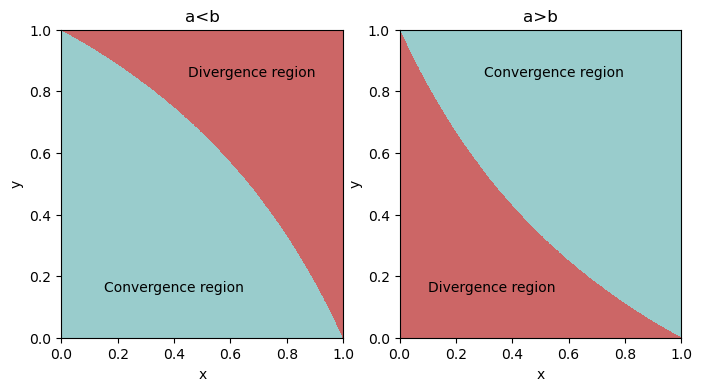
\includegraphics[width=0.6\textwidth]{Numerical/5.2.png}
	\caption{Regions of convergence and divergence for a liar Mr. N (left) and a not so liar Mr. N (right).}
	\label{fig:5.2}
\end{figure}

In the case where Mr. N is seen as trustworthy, they region of convergence is that of general agreement in that the drug is unsafe, their opinions diverging if they both believe the drug to be safe. The opposite happens whenever Mr. N is seen as a liar in general. They converge if they already kinda agreed that the pill was safe. I expected the divergence region to measure lack of agreement...

\textbf{Ex. 5.3: }It is evident from ($5.31$) that Mr. X and Mr. Y can never experience a reversal of viewpoint; that is, if initially Mr. X believes more strongly than Mr. Y in the safety of the drug, this will remain true whatever the values of $a$, $b$. Therefore, a necessary condition for reversal must be that they have different conditions about Mr. N; $a_x\neq a_y$ and/or $b_x\neq b_y$. But this does not prove that reversal is actually possible, so more analysis is needed. If reversal is possible, find a sufficient condition on $(x,\,y,\,a_x,\,a_y,\,b_x,\,b_y)$ for this to take place, and illustrate it by a verbal scenario like the above. If it is not possible, prove this and explain the intuitive reason why reversal cannot happen.

\textbf{Answer:}

The equations for the log posterior for the drug being safe now take the form
\begin{align*}
	\log\left[\frac{P(S|DI_X)}{P(\overline{S}|DI_X)}\right]&=\log\left[\frac{x}{1-x}\right]+\log\left[\frac{a_X}{b_X}\right],\\
	\log\left[\frac{P(S|DI_Y)}{P(\overline{S}|DI_Y)}\right]&=\log\left[\frac{y}{1-y}\right]+\log\left[\frac{a_Y}{b_Y}\right],
\end{align*}
so that their difference is
\begin{align*}
	\log\left[\frac{x}{1-x}\right]-\log\left[\frac{y}{1-y}\right]+\log\left[\frac{a_X}{b_X}\right]-\log\left[\frac{a_Y}{b_Y}\right].
\end{align*}

So, inversion of beliefs is acchieved by requiring that the difference of log likelihoods be greater in magnitude than the difference of original beliefs, with opposite sign. For the sake of concreteness, if $x=0.6$ and $y=0.4$, it suffices to take $a_Y/b_Y>0.6$ and $a_X/b_X<0.4$. Say, $a_Y=b_X=0.8$, $b_Y=a_X=0.2$; this takes an original degree of belief from (log prior) $0.81$ to $-1.96$.

In this example, Mr. X's belief is that the drug is most probably safe, and Mr. Y's is the opposite. But Mr. X is so convinced that Mr. N wouldn't lie, and Mr. Y is so convinced of the contrary, that their stances after this encounter become reversed. Cool.

\end{document}
\endinput
